\documentclass[11pt]{article}
\usepackage[utf8]{inputenc}
\usepackage{graphicx}
\usepackage{xcolor}
\usepackage[ngerman]{babel}
\usepackage{enumitem}
\usepackage{amsmath}
\usepackage{amsmath}
\usepackage{amsthm}
\usepackage{amssymb}
\usepackage{xcolor}
\definecolor{commentgreen}{RGB}{2,112,10}
\definecolor{eminence}{RGB}{108,48,130}
\definecolor{weborange}{RGB}{255,165,0}
\definecolor{frenchplum}{RGB}{129,20,83}
\usepackage{listings}
\lstset {
    language=Java,
    %frame=tb,
    tabsize=4,
    showstringspaces=false,
    numbers=left,
    %upquote=true,
    commentstyle=\color{commentgreen},
    keywordstyle=\color{eminence},
    stringstyle=\color{red},
    basicstyle=\small\ttfamily, % basic font setting
    emph={int,char,double,float,unsigned,void,bool},
    emphstyle={\color{blue}},
    escapechar=\&,
    % keyword highlighting
    classoffset=1, % starting new class
    otherkeywords={>,<,.,;,-,!,=,~},
    morekeywords={>,<,.,;,-,!,=,~},
    keywordstyle=\color{weborange},
    classoffset=0,
}

\graphicspath{{../images/}}

% change \iff to the shorter version
\renewcommand{\iff}{\Leftrightarrow}
\renewcommand{\implies}{\Rightarrow}

\newtheorem{theorem}{Theorem}
\newtheorem{proposition}{Proposition}
\newtheorem{lemma}{Lemma}

\setlength{\parindent}{0em}

%\author{J\"org Barkoczi}
\title{\vspace{-4.7cm}Bubble Sort}
\date{}

\begin{document}
\maketitle
\section{Grundprinzip}
Das Array wird in zwei Subarrays unterteilt: dem Sortierten und der Rest.
Pro Durchlauf wird ein Element dem sortierten Subarray hinzugef\"ugt. Dies geschieht, 
in dem immer zwei Elementpaare verglichen werden, und das Gr\"o{\ss}ere nach rechts wandert. Dies 
f\"uhrt auch dazu, dass der Algorithmus stabil ist.
\subsection{Beispiel}
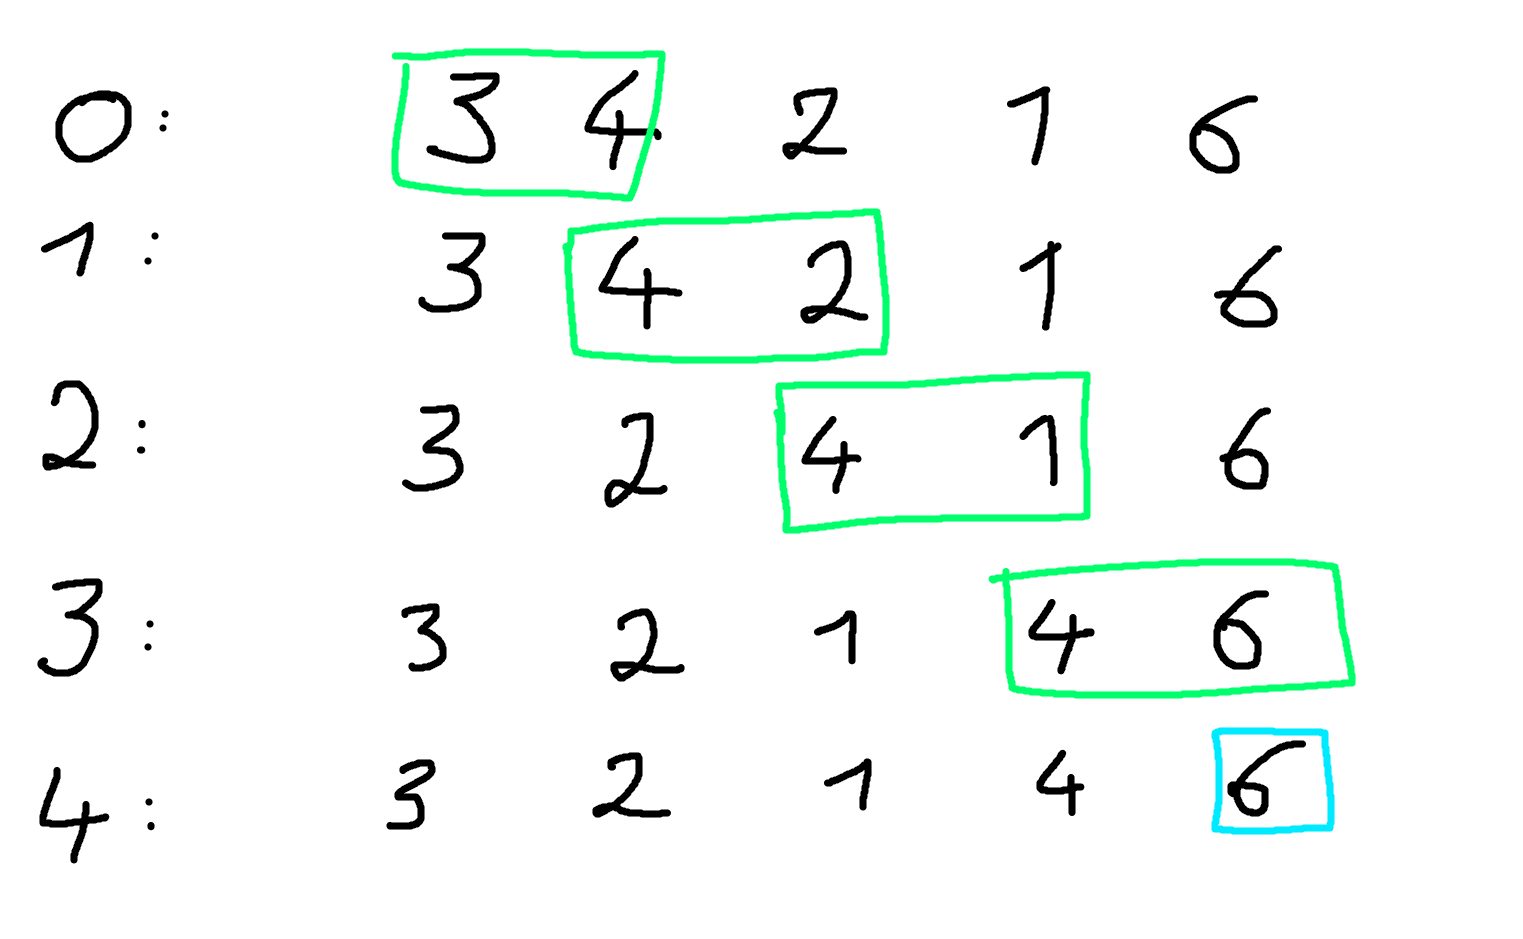
\includegraphics[scale=0.2]{qwe.png}\\
Nach diesem ersten Durchgang ist nun ein Element, die 6, im sortierten Subarray hinten.\\
Das selbe Spiel wird nun solange wiederholt, bis das sortierte Subarray alle Elemente des
urspr\"unglichen beinhalted.\\
\vspace{0.5cm}\\
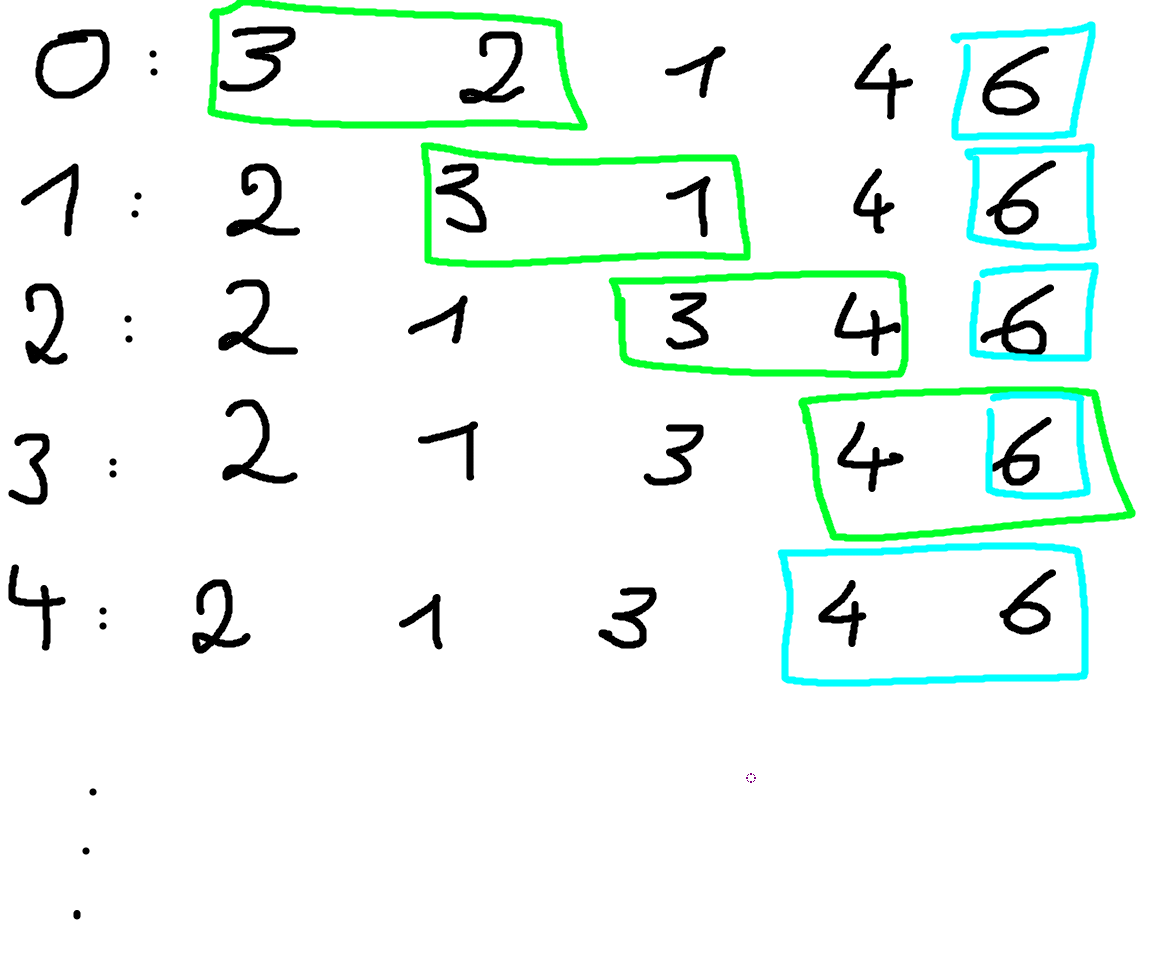
\includegraphics[scale=0.25]{qwe2.png}\\
\section{PAP}
\begin{center}
    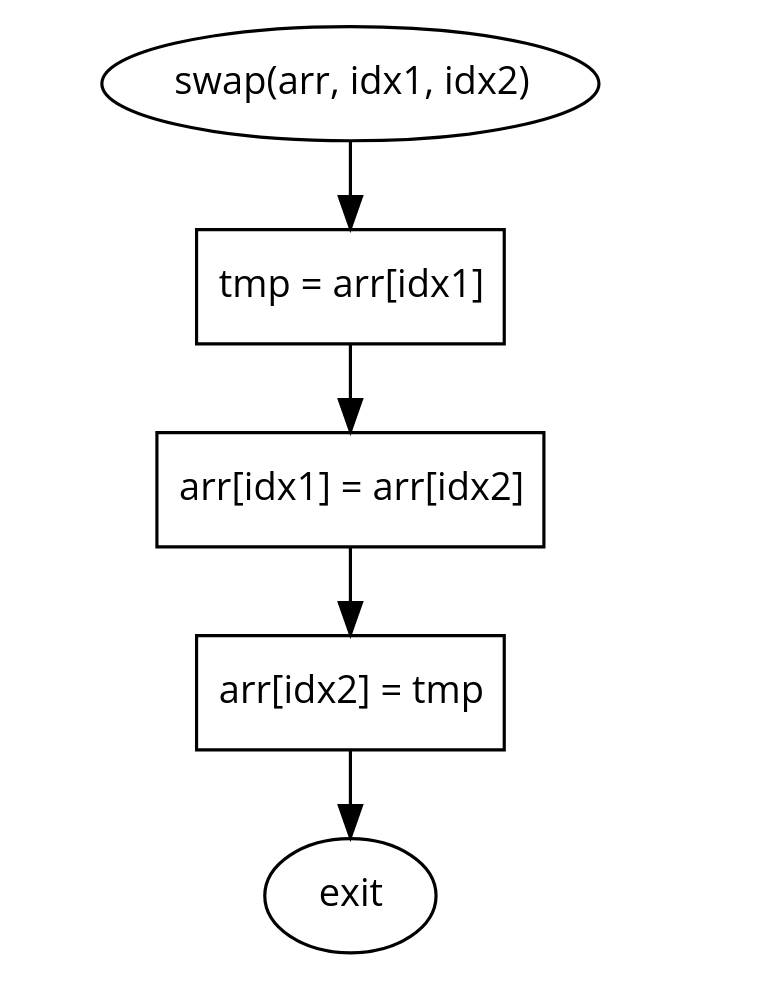
\includegraphics[scale=0.5]{swap.png}\\
\end{center}
\begin{center}
    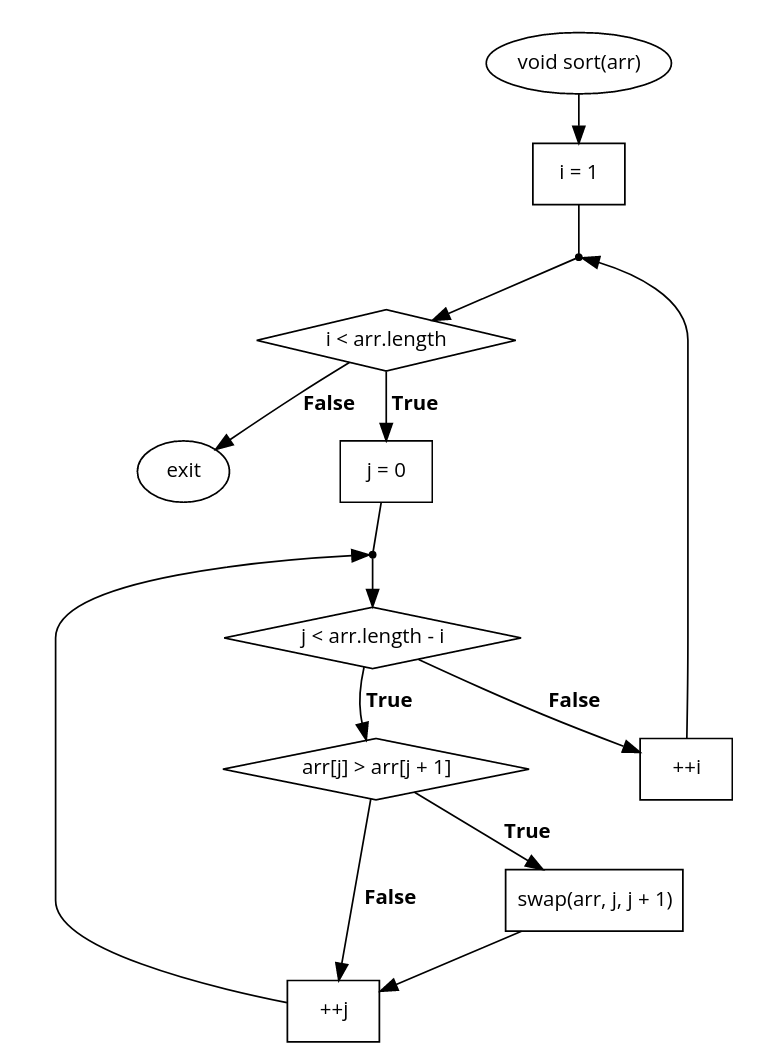
\includegraphics[scale=0.6]{sort_flow.png}\\
\end{center}
\pagebreak
\begin{center}
    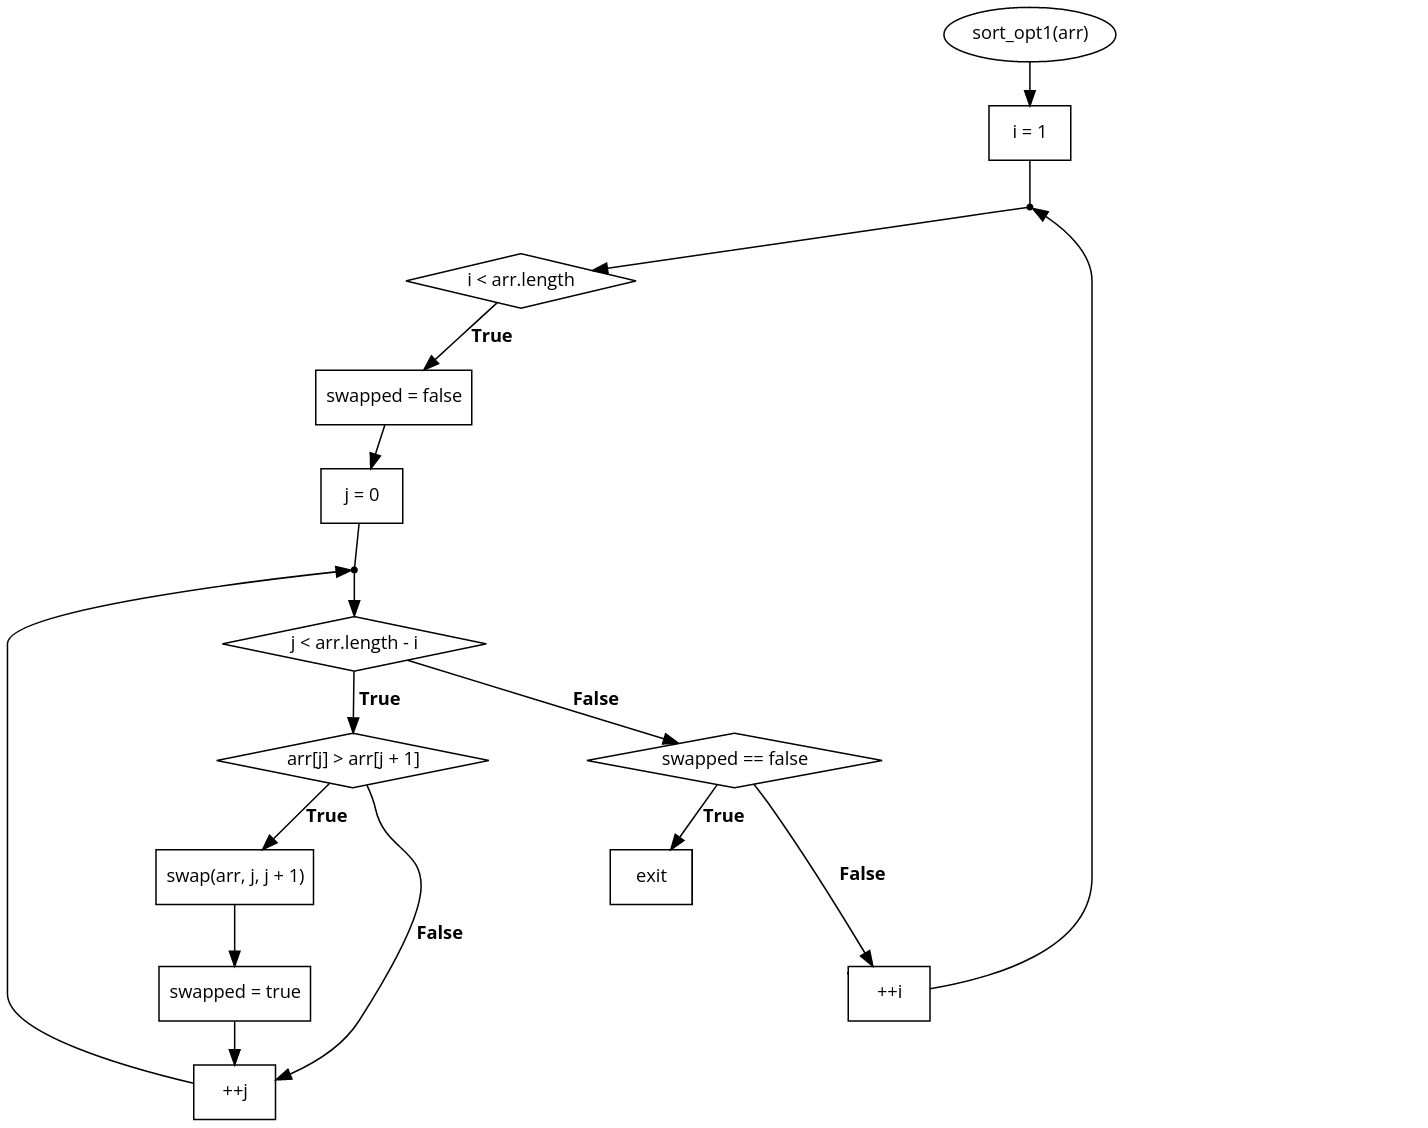
\includegraphics[scale=0.5]{sort_opt_flow.png}\\
\end{center}
\pagebreak
\section{Struktogramm}
~\\
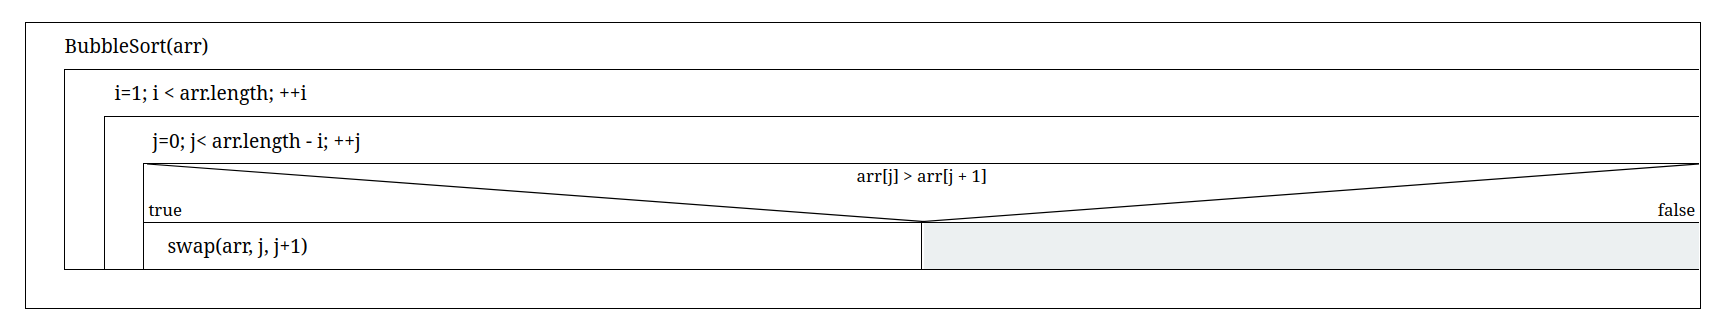
\includegraphics[scale=0.3]{sort_strukto.png}\\
\vspace{3cm}\\
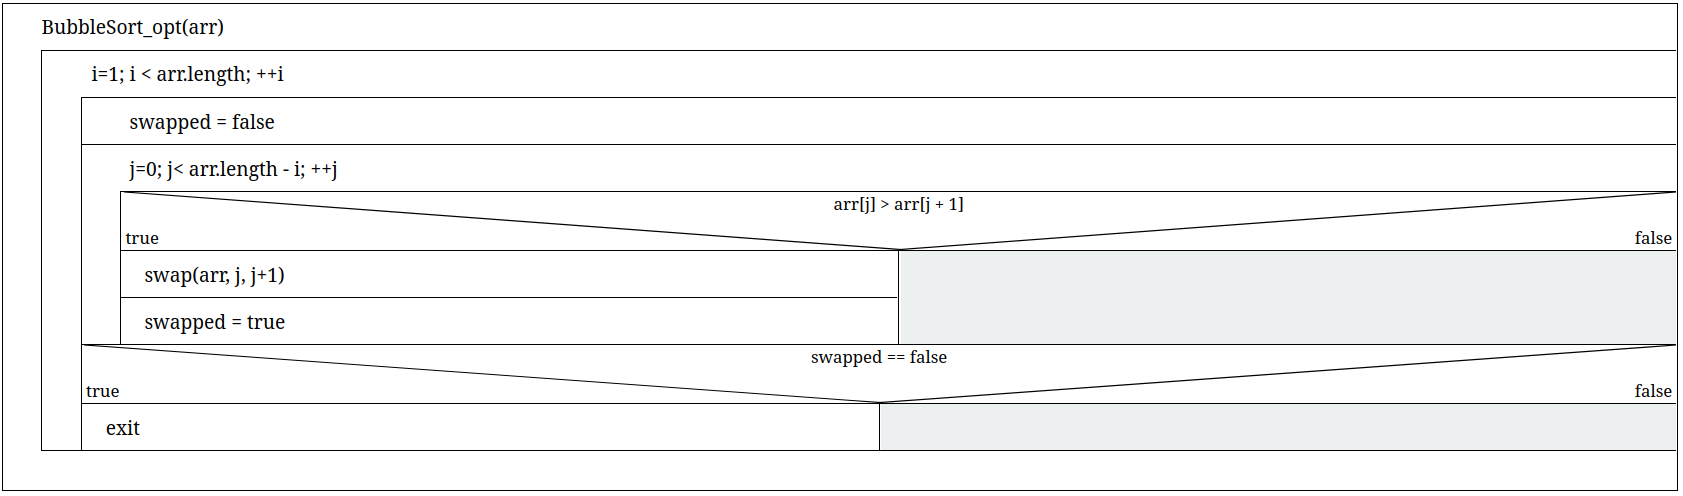
\includegraphics[scale=0.3]{sort_opt_strukto.png}\\
\pagebreak
\section{Programmierung}
\begin{lstlisting}
public static void swap(int[] arr, int idx1, int idx2)
{
    int tmp = arr[idx1];
    arr[idx1] = arr[idx2];
    arr[idx2] = tmp;
}

public static void sort(int[] arr)
{
    for (int i = 1; i < arr.length; ++i)
    {
        for (int j = 0; j < arr.length - i; ++j)
        {
            if (arr[j] > arr[j + 1])
            {
                swap(arr, j, j + 1);
            }
        }
    }
}

public static void swap(String[] arr, int idx1, int idx2)
{
    String tmp = arr[idx1];
    arr[idx1] = arr[idx2];
    arr[idx2] = tmp;
}

public static void sort(String[] arr)
{
    for (int i = 1; i < arr.length; ++i)
    {
        for (int j = 0; j < arr.length - i; ++j)
        {
            if (arr[j].compareTo(arr[j + 1]) > 0)
            {
                swap(arr, j, j + 1);
            }
        }
    }
}
\end{lstlisting}
\pagebreak

\begin{lstlisting}
public static void sort_opt1(int[] arr)
{
    for (int i = 1; i < arr.length; ++i)
    {
        boolean swapped = false;
        for (int j = 0; j < arr.length - i; ++j)
        {
            if (arr[j] > arr[j + 1])
            {
                swap(arr, j, j + 1);
                swapped = true;
            }
        }
        if (!swapped)
            break;
    }
}
\end{lstlisting}

\begin{lstlisting}
public static void sort_opt2(int[] arr)
{
    int i = arr.length - 1;
    boolean swapped = true;
    while (swapped)
    {
        swapped = false;
        int tmp_i = i;
        for (int j = 0; j < tmp_i; ++j)
        {
            if (arr[j] > arr[j + 1])
            {
                swap(arr, j, j + 1);
                swapped = true;
                i = j;
            }
        }
    }
}
\end{lstlisting}
\pagebreak

\section{Asymptotische Laufzeit-Analyse}
\subsection{Best Case}
Im Best Case ist das Array schon vorsortiert. In dem Fall haben wir mit der extra Abbruchbedingung eine 
Laufzeit von $O(n)$, also eine lineare Beziehung zwischen Arrayl\"ange und der Anzahl der Vergleichs-Operationen 
(da wegen der Abbruchbedingung, \textit{swapped}, nur einmal durchs Array gelaufen wird).
Ohne die Abbruchbedingung ist die Best Case Laufzeit \"ahnlich der Worst Case Laufzeit: Die Anzahl der Vergleichs-Operationen
steigt quadratisch zur Arrayl\"ange (siehe unten).
\subsection{Worst Case}
Im Worst Case ist das Array umgekehrt vorsortiert. In dem Fall iteriert die \"au{\ss}ere Schleife $n-1$ mal.
In jeder dieser Iteration l\"auft nun die innere Schleife erst $n-1$, dann $n-2$, \ldots, dann $1$ mal, 
wobei in jeder dieser Iterationen
eine Vergleichs- und eine Swap-Operation stattfindet. Es folgt also die folgende Beziehung $f$ zwischen der 
Arrayl\"ange $n$ und der Vergleichs- und Swap-Operationen
\begin{align*}
    f(n) &= \sum_{1}^{n-1} \left(i \cdot (V+S)\right)\\
        &= \left(\frac{n\cdot(n+1)}{2} - n\right) \cdot (V+S)\\
        &= \left(\frac{n^2-n}{2}\right) \cdot (V+S).\\
\end{align*}
Asymptotisch wird der Term $\frac{n^2-n}{2}$ von $n^2$ dominiert, es folgt also eine Worst Case Laufzeit
von $O(n^2)$.
\subsection{Average-Case} 
$O(n^2)$.

\end{document}
